 \documentclass[t]{beamer}
%\documentclass[c]{beamer}
\listfiles

\mode<presentation>
{
%  \usetheme[english,titlepage0]{KIT}
%  \usetheme[titlepage0]{KIT}
% \usetheme[usefoot]{KIT}
 \usetheme[deutsch]{KIT}

%%  \usefonttheme{structurebold}

  \setbeamercovered{transparent}

  %\setbeamertemplate{enumerate items}[circle]
  \setbeamertemplate{enumerate items}[ball]
}

\usepackage[ngerman]{babel}
\date{02. Nov 2015}
%\DateText

%\newlength{\Ku}
%\setlength{\Ku}{1.43375pt}

\usepackage[utf8]{inputenc}
\usepackage[TS1,T1]{fontenc}
\usepackage{array}
\usepackage{multicol}
\usepackage{lipsum}
\usepackage{graphicx}
\usepackage{booktabs}

\usepackage{graphics}

\usepackage{amsmath}
\usepackage{booktabs}
\usepackage{listings}

\usepackage{dot2texi}
\usepackage{tikz}
\usetikzlibrary{arrows,shapes}
 \usetikzlibrary{matrix}
\usetikzlibrary{automata}

\usepackage{wrapfig}


%\usenavigationsymbols
%\usenavigationsymbols[sfHhdb]
%\usenavigationsymbols[sfhHb]

\title{Projektvortrag Schnupperstudium}
\subtitle{KAsuro}

\author{Andreas Pfeil, Oliver Neumann}

%\institute[\raisebox{-3.5mm}{
%	\includegraphics[height=\KITlogoht]{Bilder/Zlogo}}]
%  {INSTITUTS- FAKULTÄTS-, ABTEILUNGSNAME}
%\logo{\includegraphics[width=\KITlogowd]{Bilder/Zlogo}}

\TitleImage[width=\titleimagewd]{Bilder/asuro_full}

\newcommand{\currentsection}{}
\let\oldsection\section
\renewcommand{\section}[1]{\oldsection{#1}\renewcommand{\currentsection}{#1}}


\newcommand{\currentsubsection}{}
\let\oldsubsection\subsection
\renewcommand{\subsection}[1]{\oldsubsection{#1}\renewcommand{\currentsubsection}{#1}}


\newcommand{\xn}{\visible<2->{$\times$}}
\newcommand{\xj}{\visible<2->{$\checkmark$}}
\newcommand{\rd}[1]{\textcolor{red}{#1}}
\newcommand{\gn}[1]{\textcolor{green}{#1}}
\newcommand{\bl}[1]{\textcolor{blue}{#1}}

\newcommand{\hiddencell}[2]{\action<#1->{#2}}

\newcommand{\link}[2][blue]{\underline{\textcolor{#1}{#2}}} 	% \link{www.example.org} zeigt www.example.org in blau und unterstrichen
\renewcommand{\emph}[1]{\textit{\textcolor{blue}{#1}}}			% \emph{Test} zeigt Text in blau und kursiv
\newcommand{\warn}[1]{\textcolor{red}{#1}}			% \warn{Warning} zeigt Warning in rot und kursiv
\begin{document}

\begin{frame}
\maketitle
\end{frame}

\section{Einleitung}
\subsection{Begrüßung}
\begin{frame}
	\frametitle{\currentsection}
	\framesubtitle{\currentsubsection}
  \begin{block}<1->{Wer sind wir?}
  \begin{itemize}
  	\item Andreas Pfeil
  	\begin{itemize}
  		\item Informatik 9. Semester
  		\item aus Badisch-Sibirien
  		\item ...
  	\end{itemize}
  	\item Oliver Neumann
	\begin{itemize}
		\item Informatik 7. Semester
		\item aus Aalen
		\item ...
	\end{itemize}
  \end{itemize}
  \end{block}
\end{frame}
\begin{frame}
	\frametitle{\currentsection}
	\framesubtitle{\currentsubsection}
	\begin{block}<1->{Wer seid ihr?}
		\begin{itemize}
			\item Name?
			\item Herkunft?
			\item Hobbies?
			\item Erfahrungen?
		\end{itemize}
	\end{block}
\end{frame}


\subsection{Hinweis!}
\begin{frame}[c]
	\frametitle{\currentsection}
	\framesubtitle{\currentsubsection}
	\centering \Huge Fragen sind jederzeit erwünscht!
\end{frame} 
\section{Projekt}
\subsection{Wochenplan}
\begin{frame}
	\frametitle{\currentsection}
	\framesubtitle{\currentsubsection}
	\only<1> {
		\begin{block}{Tag 1}
			\begin{itemize}
				\item Vortrag (jetzt!)
				\item Einteilung in Gruppen
				\item Austeilung der Asuros
				\item Austeilung der Notebooks
				\item Erstes Programm
				\item (Aufgabe überlegen)
			\end{itemize}
		\end{block}
	}
	\only<2> {
		\begin{block}{Tag 2}
			\begin{itemize}
				\item Parametrisierung
				\item Projektarbeit
			\end{itemize}
		\end{block}
		\begin{block}{Tag 3-4}
			\begin{itemize}
				\item Projektarbeit
			\end{itemize}
		\end{block}
		\begin{block}{Tag 5}
			\begin{itemize}
				\item Feinschliff und Präsentation
			\end{itemize}
		\end{block}
	}
\end{frame}


\subsection{Mögliche Projekte}
\begin{frame}[c]
	\frametitle{\currentsection}
	\framesubtitle{\currentsubsection}
	\begin{itemize}
		\item ''Morsen'': Benutzt Lichtsignale um von einem zum anderen Asuro Informationen zu übertragen.
		\item ''Musiker'': Benutzt das piepsen der Motoren um Töne zu erzeugen.
		\item ''Linienfolger'': Findet und folgt einer Linie, indem ihr die Lichtsensoren nutzt.
		\item ''Strichcode-Leser'': Der Asuro muss die Anzahl der Linien zählen die er überfährt.
		\item ''Lebewesen'': Ist Asuro Lichtscheu oder fühlt er sich davon angezogen? Müde oder hellwach? Versucht den Asuro lebendig wirken zu lassen.
		\item ''Fernbedienung'': Der Asuro muss den Befehlen des Computers folgen.		
	\end{itemize}
\end{frame}
\section{C-Einführung}
\subsection{Verständnis}
\begin{frame}
	\frametitle{\currentsection}
	\framesubtitle{\currentsubsection}
	\begin{block}<1->{Was ist ein Programm?}
		\begin{itemize}
			\item C Datei als Beschreibung des Programms
			\item Compilieren der C Datei mit Compiler zu Assembler
			\item Assembler stellen 1:1 die Befehle der CPU dar
			\item Übersetzen von Assembler nach Hex
			\item Aufspielen der Hex über Flasher
		\end{itemize}
	\end{block}
\end{frame}


\subsection{Funktionen}
\begin{frame}
	\frametitle{\currentsection}
	\framesubtitle{\currentsubsection}
	\begin{block}<1->{Was ist eine Funktion?}
		\begin{itemize}
			\item Strukturieren Programme
			\item Beschreiben den Einstiegspunkt (main Funktion)
			\item Sind ähnlich zu mathematischen Funktionen
			\item Können Werte zurückliefern aber auch Werte benötigen
		\end{itemize}
	\end{block}
\end{frame}
\begin{frame}
	\frametitle{\currentsection}
	\framesubtitle{\currentsubsection}
  \begin{block}<1->{Beispiele}
  	\lstinputlisting[language=C]{Code/Examples/function.c}
  \end{block}
\end{frame}


\subsection{Variablen}
\begin{frame}
	\frametitle{\currentsection}
	\framesubtitle{\currentsubsection}
	\begin{block}<1->{Wie merke ich mir Dinge?}
		\begin{itemize}
			\item Variablen sind dafür gedacht Werte zu speichern.
			\item Variablen haben IMMER einen Typ und einen Namen!
			\item Es gibt unter anderem folgende Typen:
			\begin{itemize}
				\item int, long
				\item float, double
				\item char
			\end{itemize}
		\end{itemize}
	\end{block}
\end{frame}
\begin{frame}
	\frametitle{\currentsection}
	\framesubtitle{\currentsubsection}
	\begin{block}<1->{Beispiele}
		\lstinputlisting[language=C]{Code/Examples/variable.c}
	\end{block}
\end{frame}

\subsection{Operationen}
\begin{frame}
	\frametitle{\currentsection}
	\framesubtitle{\currentsubsection}
	\begin{block}<1->{Beispiele}
		\lstinputlisting[language=C]{Code/Examples/operations.c}
	\end{block}
\end{frame}


\subsection{Verzweigungen}
\begin{frame}
	\frametitle{\currentsection}
	\framesubtitle{\currentsubsection}
	\begin{block}<1->{Wie entscheide Dinge?}
		\begin{itemize}
			\item Um Entscheidungen zu treffen gibt es
			\begin{itemize}
				\item if ([COND]) else
				\item switch
			\end{itemize}
		\end{itemize}
	\end{block}
\end{frame}
\begin{frame}
	\frametitle{\currentsection}
	\framesubtitle{\currentsubsection}
	\begin{block}<1->{Beispiele}
		\lstinputlisting[language=C]{Code/Examples/branch.c}
	\end{block}
\end{frame}


\subsection{Schleifen}
\begin{frame}
	\frametitle{\currentsection}
	\framesubtitle{\currentsubsection}
	\begin{block}<1->{Wie wiederhole ich Dinge?}
		\begin{itemize}
			\item Schleifen vermeiden redundanten Code
			\begin{itemize}
				\item z.B. Eine Liste durchgehen, ...
			\end{itemize}
			\item In C gibt es
			\begin{itemize}
				\item while ([COND])
				\item for (i=0; [COND]; i++)
			\end{itemize}
		\end{itemize}
	\end{block}
\end{frame}
\begin{frame}
	\frametitle{\currentsection}
	\framesubtitle{\currentsubsection}
	\begin{block}<1->{Beispiele}
		\lstinputlisting[language=C]{Code/Examples/loops.c}
	\end{block}
\end{frame}


\subsection{Compiler Stuff ... -.-}
\begin{frame}
	\frametitle{\currentsection}
	\framesubtitle{\currentsubsection}
	\begin{block}<1->{Includes}
		\begin{itemize}
			\item Funktionen/Dateien einbinden
			\begin{itemize}
				\item \#include ''somefoo.h''
				\item \#include <asuro.h>
				\item \#include <stdio.h>
				\item \#include <Math.h>
			\end{itemize}
		\end{itemize}
	\end{block}
	\begin{block}<2->{Defines}
		\begin{itemize}
			\item Variablen definieren
			\begin{itemize}
				\item \#define PI 3.14159265359
				\item \#define OUT "Some output"
				\item \#define SWITCH(X) 1<<X
			\end{itemize}
		\end{itemize}
	\end{block}
\end{frame}
\section{Asuro}
\subsection{Aufbau}
\begin{frame}[c]
	\frametitle{\currentsection}
	\framesubtitle{\currentsubsection}
	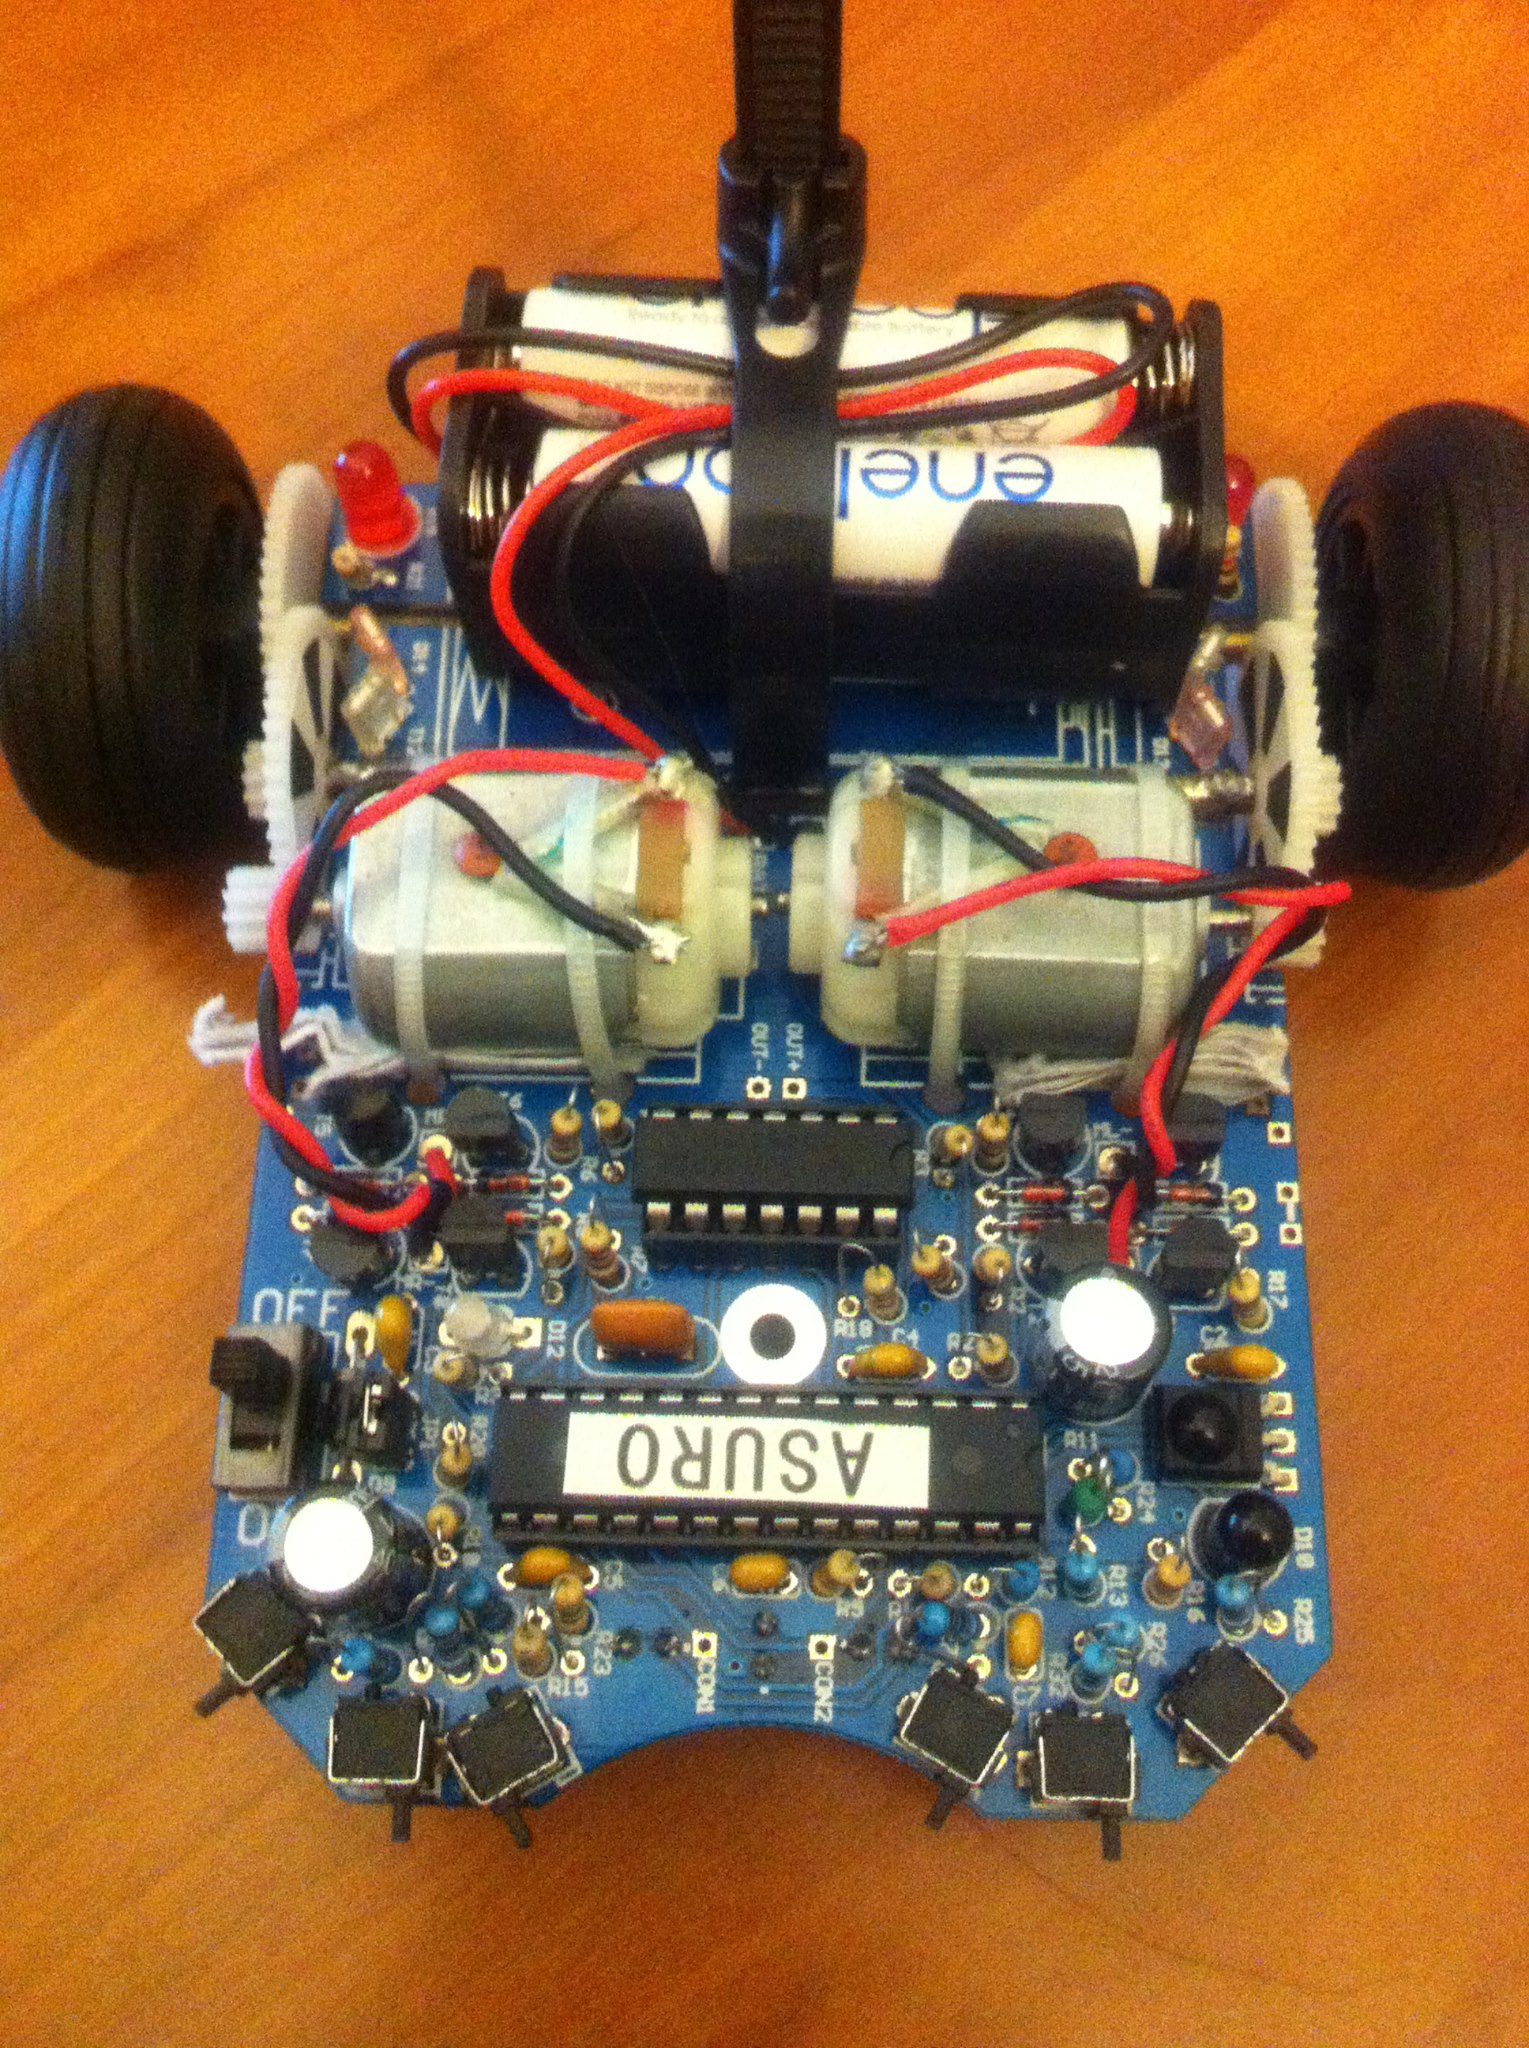
\includegraphics[scale=0.125, angle=90, origin=c]{Bilder/asuro_top}
\end{frame}
\begin{frame}[c]
	\frametitle{\currentsection}
	\framesubtitle{\currentsubsection}
	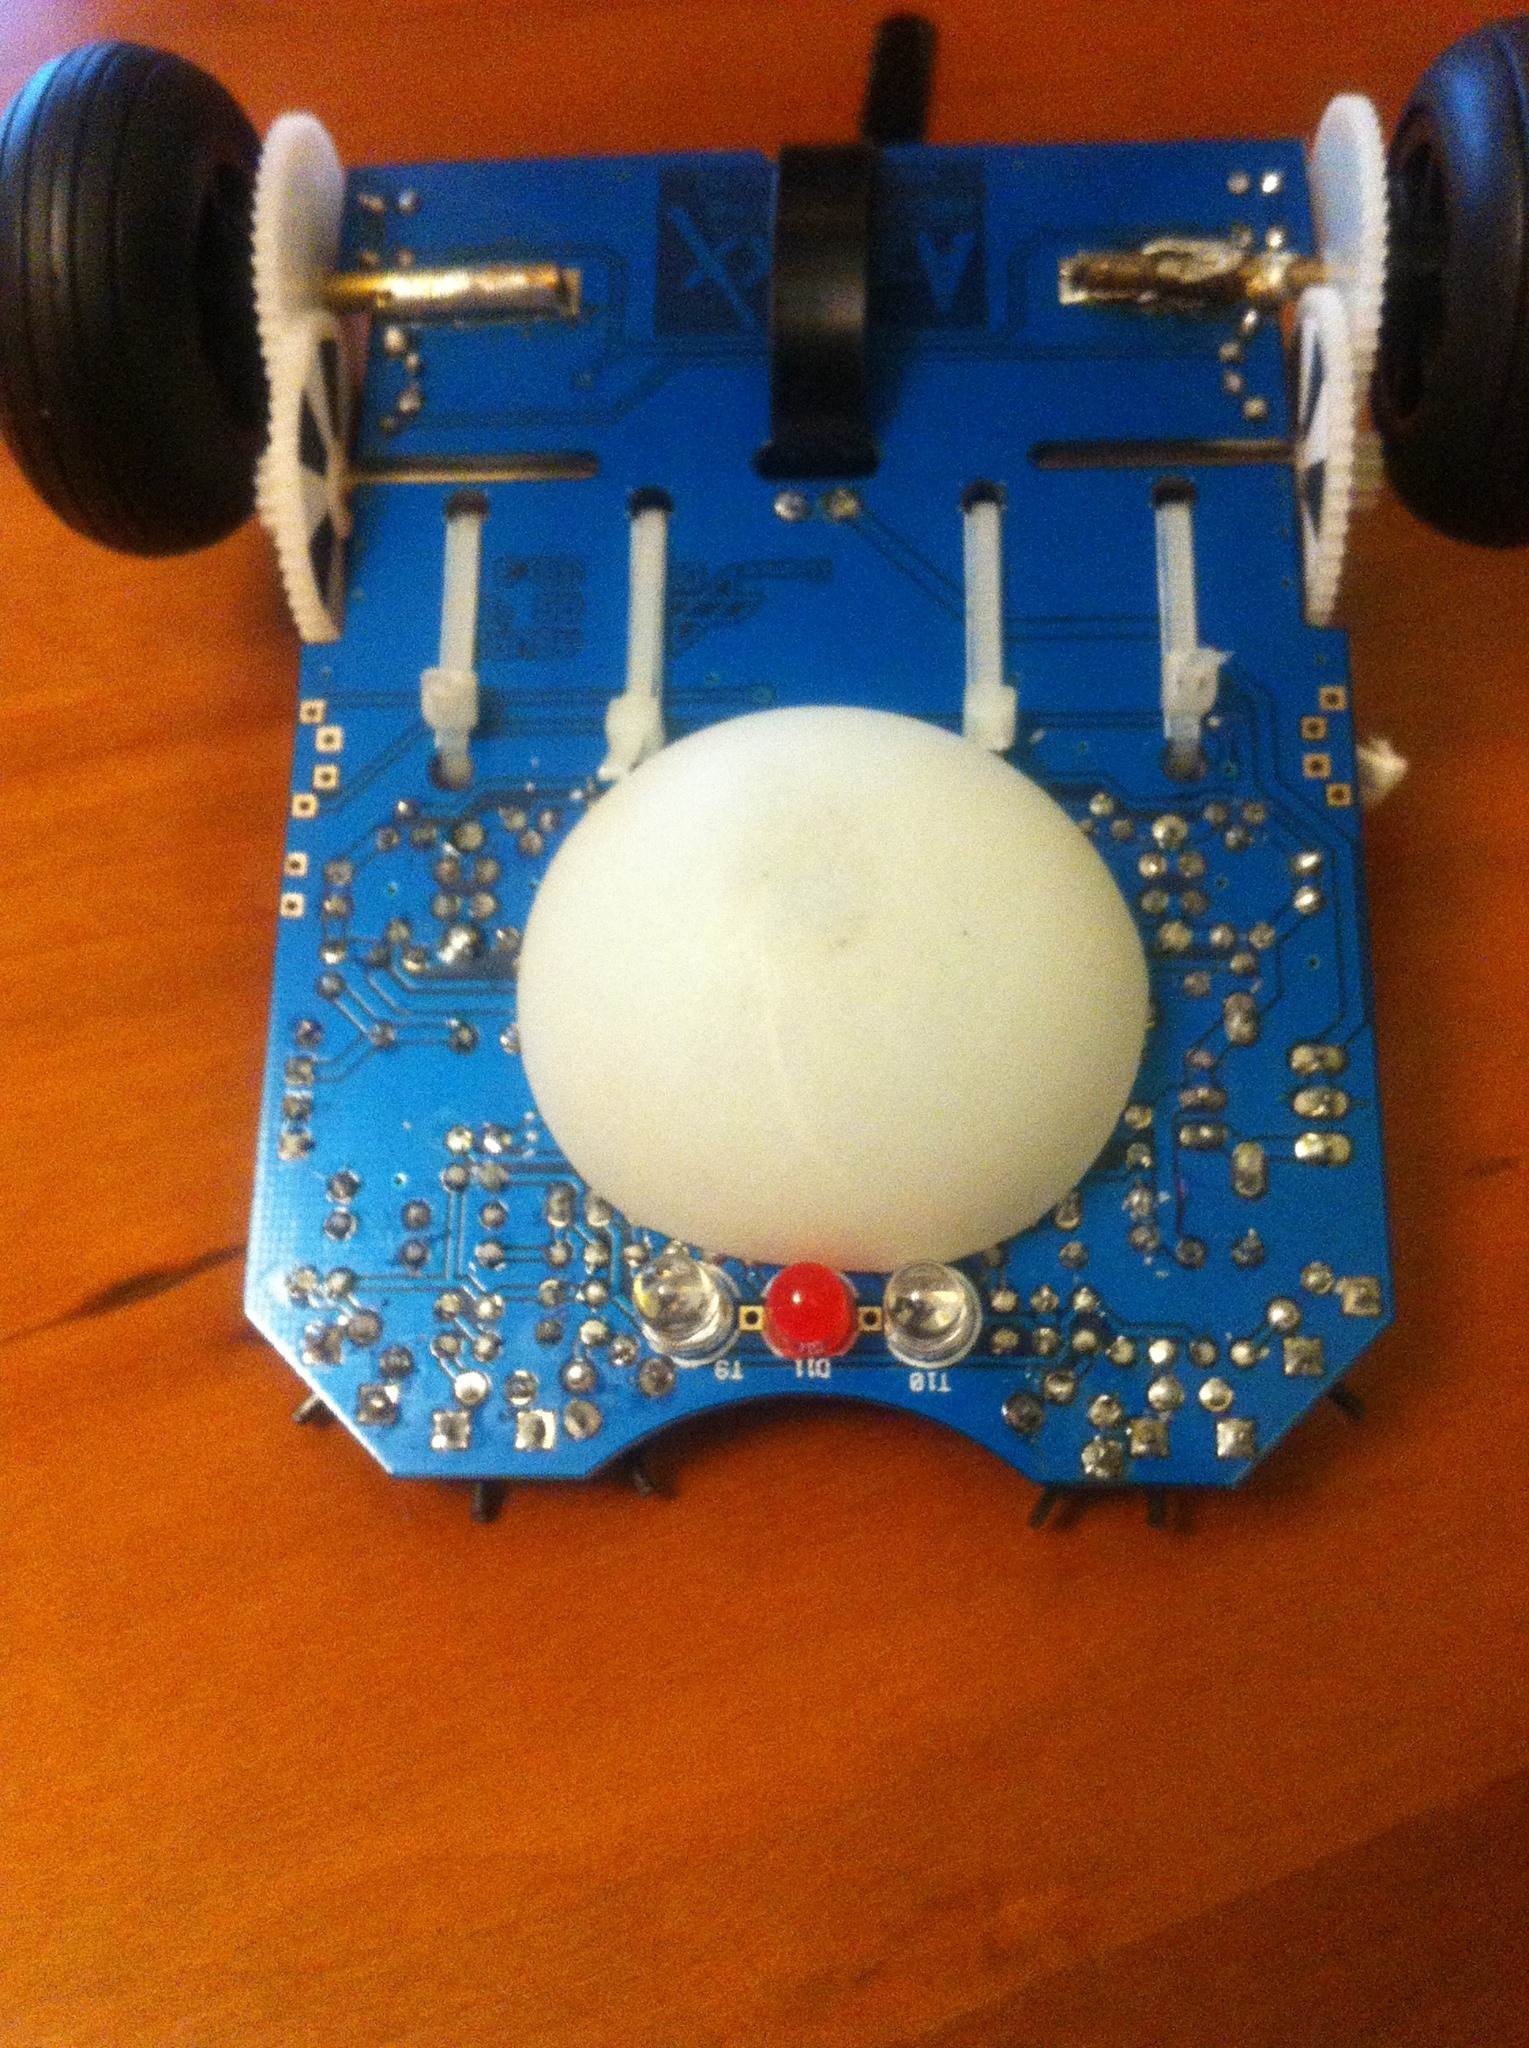
\includegraphics[scale=0.125, angle=90, origin=c]{Bilder/asuro_bottom}
\end{frame}


\subsection{Library}
\begin{frame}[c]
	\frametitle{\currentsection}
	\framesubtitle{\currentsubsection}
	\begin{block}<1->{Wichtige Funktionen}
		\begin{itemize}
			\item void Init();
			\item void GoTurn(int16\_t distance, int16\_t degree, uint8\_t speed);
			\item void BackLED(const uint8\_t left, const uint8\_t right);
			\item void FrontLED(const uint8\_t status);
			\item void StatusLED(const uint8\_t color);
			\item void MotorDir(const uint8\_t left\_dir, const uint8\_t right\_dir);
			\item void MotorSpeed(const uint8\_t left\_speed, const uint8\_t right\_speed);
			\item void LineData(uint16\_t * const data);
			\item uint8\_t PollSwitch(void);
			\item void msleep(uint16\_t ms);
		\end{itemize}
	\end{block}
\end{frame}


\subsection{Beispiel Programm}
\begin{frame}[c]
	\frametitle{\currentsection}
	\framesubtitle{\currentsubsection}
	\lstinputlisting[language=C]{Code/Examples/example.c}
\end{frame}

\begin{frame}[c]
	\centering \Huge Ein- und Verteilung
\end{frame}

\begin{frame}[c]
	\centering \Huge Los geht's mit Vorführung! :)
\end{frame}

\end{document}
